\documentclass[dvipsnames]{beamer}
\usepackage{lmodern}
\usepackage{appendixnumberbeamer}
\renewcommand{\sfdefault}{lmss}
\renewcommand{\ttdefault}{lmtt}
\usepackage[T1]{fontenc}
% \usepackage[utf8]{inputenc}
\setcounter{secnumdepth}{3}
\setcounter{tocdepth}{3}
\usepackage{amsmath}
\usepackage{amsthm}
\usepackage{amssymb}
\theoremstyle{definition}
\newtheorem*{defn*}{\protect\definitionname}
\providecommand{\definitionname}{Definition}
\usepackage{graphicx}
\usepackage{hyperref}
\usepackage{ulem}
\PassOptionsToPackage{normalem}{ulem}
\usepackage{caption}
\usepackage{subcaption}
\usepackage{verbatim}
\usepackage[english]{babel}
\usepackage[autostyle]{csquotes}
\usepackage{tikz}
\usetikzlibrary{arrows,intersections}
\usepackage{pgfplots}
\pgfplotsset{compat = 1.15}
\usepgfplotslibrary{fillbetween}
\usepackage{verbatim}
\usepackage{booktabs}
\usepackage{multirow}
\usepackage{array}
\usepackage{nccmath}
% \usepackage{listings}
\usepackage{mathtools}

%Bibliography style, etc.
\usepackage[citestyle=authoryear-comp,natbib, uniquename = false, url = false, doi = false, uniquelist=false]{biblatex}
\renewbibmacro{in:}{}
\AtEveryBibitem{%
  \clearfield{volume}%
  \clearfield{number}
  \clearfield{month}
  \clearfield{issn}
  \clearfield{isbn}
  \clearfield{pages}
}

%\usepackage{cleveref}
\usepackage{setspace}
\makeatletter

% Macros
\providecommand{\tabularnewline}{\\}
\newcommand{\gr}{\textcolor{ForestGreen}} 
\newcommand{\rd}{\textcolor{red}}
\newcommand{\cb}{\textcolor{CornflowerBlue}} %this is the blue color you like; simply type \cb{X} where "X" is the color you want in blue
\newcommand{\vitem}{\vfill \item} %auto-centers items in lists
\newcommand{\fall}{\ \forall} %redefines "forall" (I don't like the default spacing)
\newcommand{\frall}{\quad \forall} %a \forall separated from the main math; this is the way it usually shows up in equations
\newcommand{\exist}{\ \exists} %same as \fall, but for \exists; they have the same ugly spacing
\newcommand{\R}{\mathbb{R}} %set of real numbers
\newcommand*\bigcdot{\mathpalette\bigcdot@{.5}} %different size for cdots
% \newcommand{\argmax}{\text{arg}\max}
\newenvironment{itemframe}
    {\frame{}\itemize}
    {\itemize\frame}
\newcommand\makebeamertitle{\frame{\maketitle}}%
\newtheoremstyle{named}{}{}{\itshape}{}{\bfseries}{.}{.5em}{\thmnote{#3's }#1}
\theoremstyle{named}
\newtheorem*{prop*}{Proposition}
% \newtheorem*{corollary}{Corollary}
\newtheorem*{namedtheorem}{Theorem} %allows named theorems
\newtheorem*{nameddef}{Definition}
\newtheorem{proposition}{Proposition}
\newtheorem*{assumption}{Assumption}
\newtheorem*{namedcorollary}{Corollary}
\newtheorem*{namedlemma}{Lemma}
\newtheorem*{axiom}{Axiom}
\newtheorem*{theorem*}{Theorem}
\newtheorem*{lemma*}{Lemma}
\DeclareMathOperator*{\argmin}{argmin}
\DeclareMathOperator{\argmax}{argmax}
\DeclareMathOperator{\supp}{supp}
\DeclareMathOperator{\interior}{int}
\DeclareMathOperator{\rank}{rank}
\newcolumntype{C}[1]{>{\centering\let\newline\\\arraybackslash\hspace{0pt}}m{#1}}
\newcommand{\sbt}{\,\begin{picture}(-1,1)(-1,-3)\circle*{2}\end{picture}\ }



%formatting
\usetheme{Ilmenau}
\definecolor{MIT}{rgb}{.639,.122,.204}
\definecolor{UCLA}{rgb}{0.15294117647058825, 0.4549019607843137, 0.6823529411764706}
\definecolor{UCLA_gold}{rgb}{1, 0.8196078431372549, 0}
\usecolortheme[named=UCLA]{structure}
\setbeamercolor*{palette secondary}{fg=UCLA_gold,bg=gray!15!white}
\usecolortheme{dolphin}
\setbeamertemplate{navigation symbols}{} 
\setbeamertemplate{footline}{}{}
\setbeamertemplate{headline}{}
\setbeamertemplate{navigation symbols}{}
\mode<presentation> {}
\setbeamercolor{block title}{use=structure,fg=white,bg=RoyalBlue} %blocks (theorems, etc.)in blue
\setbeamercolor{block title alerted}{use=structure,fg=white,bg=ForestGreen} %blocks (theorems, etc.)in blue

\renewcommand\qedsymbol{$\blacksquare$} %set QED symbol as black square
\renewcommand{\emph}{\textit} %set emphasized text style; this is italics
\setbeamertemplate{footline}[frame number] %slide numbers
\setbeamertemplate{itemize item}[circle] %bullet style
\setbeamertemplate{itemize subitem}{--}
\setbeamertemplate{enumerate item}[default]
\newrobustcmd*{\parentexttrack}[1]{%
  \begingroup
  \blx@blxinit
  \blx@setsfcodes
  \blx@bibopenparen#1\blx@bibcloseparen
  \endgroup}

\AtEveryCite{%
  \let\parentext=\parentexttrack%
  \let\bibopenparen=\bibopenbracket%
  \let\bibcloseparen=\bibclosebracket}

 \AtBeginDocument{%
   \let\origtableofcontents=\tableofcontents
   \def\tableofcontents{\@ifnextchar[{\origtableofcontents}{\gobbletableofcontents}}
   \def\gobbletableofcontents#1{\origtableofcontents}
 }
\newcommand{\backupbegin}{
   \newcounter{framenumberappendix}
   \setcounter{framenumberappendix}{\value{framenumber}}
}
\newcommand{\backupend}{
   \addtocounter{framenumberappendix}{-\value{framenumber}}
   \addtocounter{framenumber}{\value{framenumberappendix}} 
} 

\renewcommand{\maketitle}{
\setbeamertemplate{footline}{} 
\begin{frame}[noframenumbering]
\titlepage
\end{frame}
\setbeamertemplate{footline}[frame number]
}

\usefonttheme[onlymath]{serif}

% \usetheme{CambridgeUS}

% \newtheorem{theorem}{Theorem}
% \theoremstyle{claim}
\newtheorem{claim}{Claim}
% \newtheorem{corollary}{Corollary}


\makeatother


%\author{Drew Fudenberg}

\institute[]{}
\usepackage{ragged2e} %justify text
\newcommand{\var}{\operatorname{Var}}
\title{The Network Origins of Aggregate Fluctuations\\
  Acemoglu, Carvalho, Ozdaglar \& Tahbaz-Salehi\\
  \emph{Econometrica 2012}
}
\author{Chris Ackerman and Antonio Martner}

\begin{document}
\maketitle

\begin{frame}
\frametitle{Motivation (1)}
\justifying

{\bf Question:}\\
Do microeconomic sector specific shocks lead to aggregate fluctuations in 
presence of heterogenous intersectoral input–output linkages?\\
\vspace{0.5cm}
{\bf What this paper do:}
\begin{itemize}
  \item Develops a multisector model that captures input–output linkages.
  \item Propose three 3 key theorems to describe how idiosyncratic shocks propagate
  and average out.
  \item Provide an evidence based application of the theory developed.
\end{itemize}

\end{frame}
%%%%%%%%%%%%%%%%%%%%%%%%%
\begin{frame}
    \frametitle{Motivation (2)}
    \justifying
    {\bf Why is this important:}\\
    Independent shocks to specific industries do not vanish as quickly as the
    previous literature proposed, generating more persistent effects that initially
    thought.\\
\vspace{0.5cm}
{\bf Key inside:}\\
Microeconomic shocks effects may not remain confined
to where they originate.\\
$\implies$ Microeconomic shocks may propagate
throughout the economy, affect the output of other sectors, and generate sizable
aggregate effects.\\
\vspace{0.5cm}
    {\bf Main contribution:}\\
    Provide a mathematical
    framework for the analysis of shocks propagations and to characterize
    that their role in aggregate fluctuations depend on the structure of 
    interactions between different sectors.
    
    \end{frame}
%%%%%%%%%%%%%%%%%%%%%%%%%
%\begin{frame}
 %   \frametitle{Table of Contents}
  %  \tableofcontents
%\end{frame}

%%%%%%%%%%%%%%%%%%%%%%%%%


\begin{frame}{Previous argument}
    \justifying
    Idiosyncratic shocks generate that aggregate output concentrates around its mean at a very rapid rate.\\[5pt]
    $\implies$  In an economy consisting of n sectors hit by independent shocks, aggregate fluctuations 
    would have a magnitude proportional to $1/ \sqrt{n}$\\[5pt]
    $\implies$ Negligible effect at
    high levels of disaggregation.\\[10pt]
    
    This argument ignores the presence of interconnections between
    different firms and sectors, functioning as a potential propagation mechanism
    of idiosyncratic shocks throughout the economy.\\
\end{frame}
%%%%%%%%%%%%%%%%%%%%%%%%%


\begin{frame}{Real life statement}
    \justifying
    Ford's CEO requested emergency government support for General Motors and
    Chrysler in nov 2008 (Why in the world he will do that?)\\[10pt]
    
    He argued that, given the significant
    overlap in the suppliers and dealers of the three automakers, the collapse of
    either GM or Chrysler would have a ripple effect across the industry, leading
    to severe disruption of Ford’s production operations within days, if not hours.\\
\end{frame}

%%%%%%%%%%%%%%%%%%%%%%%%%
\begin{frame}{Graph examples: Previous argument works}
    \justifying
   As n increases and the economy becomes more disaggregated,
    the diversification argument based on the LLN
    implies that independent sectoral shocks average out rapidly at the rate
    $\sqrt{n}$.
    
    \begin{figure}[H]
      \caption*{Symmetric economies}
      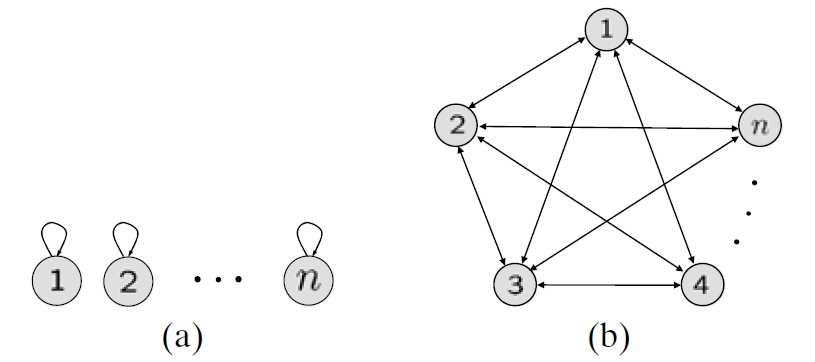
\includegraphics[scale=0.7]{1}
      \centering
    \end{figure}

The symmetric
structure of this economy ensures that aggregate output is a symmetric
function of the shocks to each sector, implying that the diversification argument
remains applicable.

\end{frame}
%%%%%%%%%%%%%%%%%%%%%%%%%
\begin{frame}{Graph examples: Previous argument NOT works}
    \justifying
    Consider  an economy with small number of sectors playing a disproportionately
    important role as input suppliers to others. Consequently, the
    interplay of sectoral shocks and the intersectoral network structure may generate
    sizable aggregate fluctuations.
    
    \begin{figure}[H]
      \caption*{One sector is the only supplier of all other sectors}
      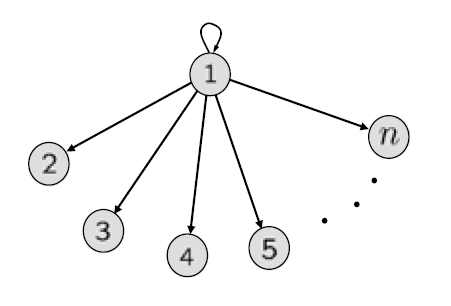
\includegraphics[scale=0.7]{2}
      \centering
    \end{figure}
\end{frame}

%%%%%%%%%%%%%%%%%%%%%%%%%
\begin{frame}{How real graphs look}
    \justifying
    \begin{figure}[H]
        \caption*{Network corresponding to the U.S. input–output matrix in 1997}
        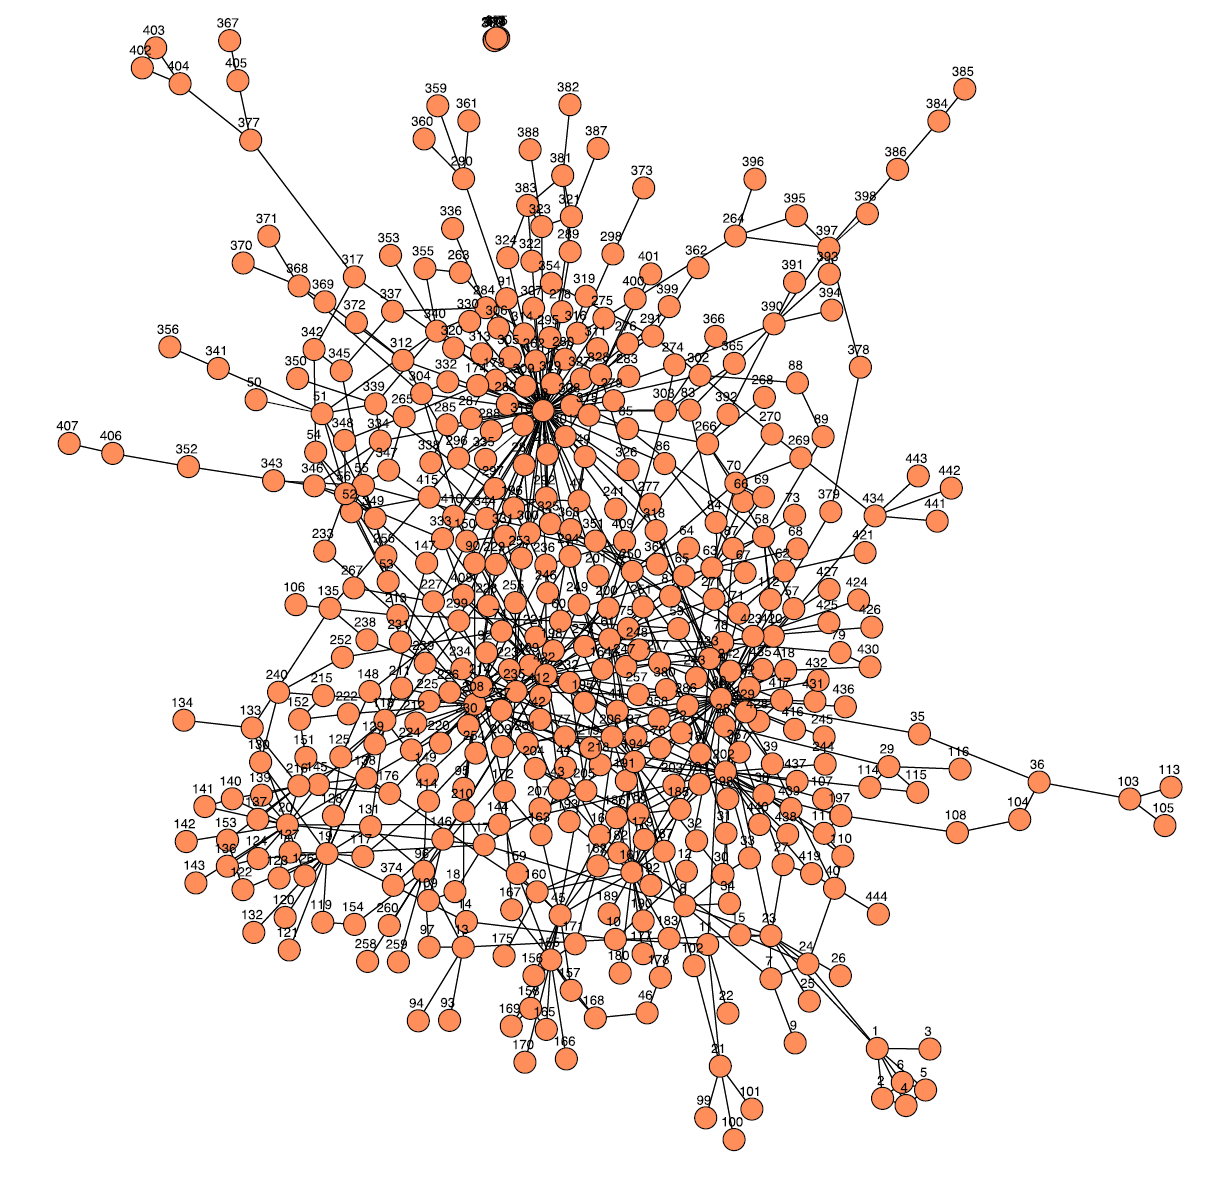
\includegraphics[scale=0.4]{3}
        \centering
      \end{figure}   

      $\implies$  Small number of sectors playing a disproportionately
      important role as input suppliers to others
\end{frame}

%%%%%%%%%%%%%%%%%%%%%%%%%
\begin{frame}{Road map}
    \justifying    

    Investigate whether aggregate volatility, defined as the standard deviation of log
    output, vanishes as $n\rightarrow\infty$.\\[10pt]
    \begin{itemize}
        \justifying    
        \item In certain cases, such as the star network,
        the LLN fails and aggregate output does not concentrate
        around a constant value.
        \item The main focus, however, is on the more interesting cases
        in which the law of large numbers holds, yet the structure of the intersectoral
        network still has a defining effect on aggregate fluctuations.
        \item  Sectoral interconnections may imply that aggregate output concentrates around its
        mean at a rate significantly slower than $\sqrt{n}$.
    \end{itemize} 

    \end{frame}

%%%%%%%%%%%%%%%%%%%%%%%%%
\begin{frame}{Model}
    \justifying
  
\end{frame}

%%%%%%%%%%%%%%%%%%%%%%%%%
\begin{frame}{Theorems}
    \justifying
  
\end{frame}

%%%%%%%%%%%%%%%%%%%%%%%%%
\begin{frame}{Application: Setup}
    \justifying
  {\bf Data:} Detailed
  benchmark input–output accounts spanning the 1972–2002 period, compiled
  every five years by the Bureau of Economic Analysis.\\[5pt]
\begin{figure}[H]
    \caption*{ Intermediate input intensity shares:}
    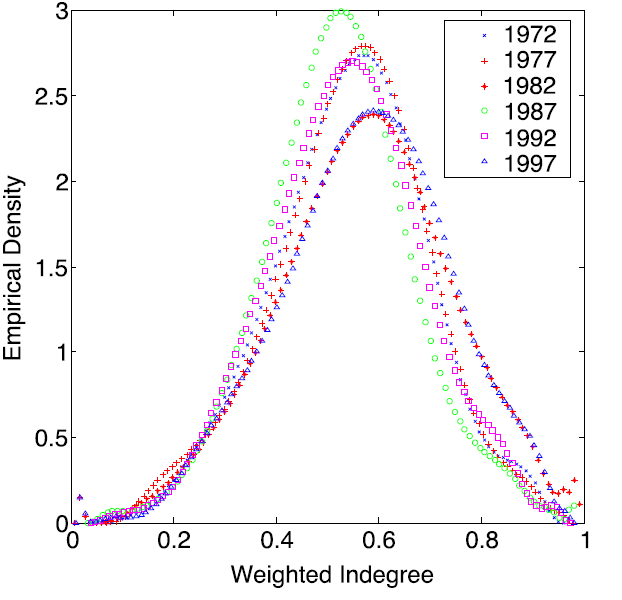
\includegraphics[scale=0.6]{4}
    \centering
\end{figure}   

$\implies$ Most sectors are concentrated around the mean (0.55).: on average, 71\% of the sectors are within one
standard deviation of the mean input share.
\end{frame}

%%%%%%%%%%%%%%%%%%%%%%%%%
\begin{frame}{First- and second-order OUT-degrees densities}
    \justifying
    \begin{figure}[H]
        \caption*{ Intermediate input intensity shares:}
        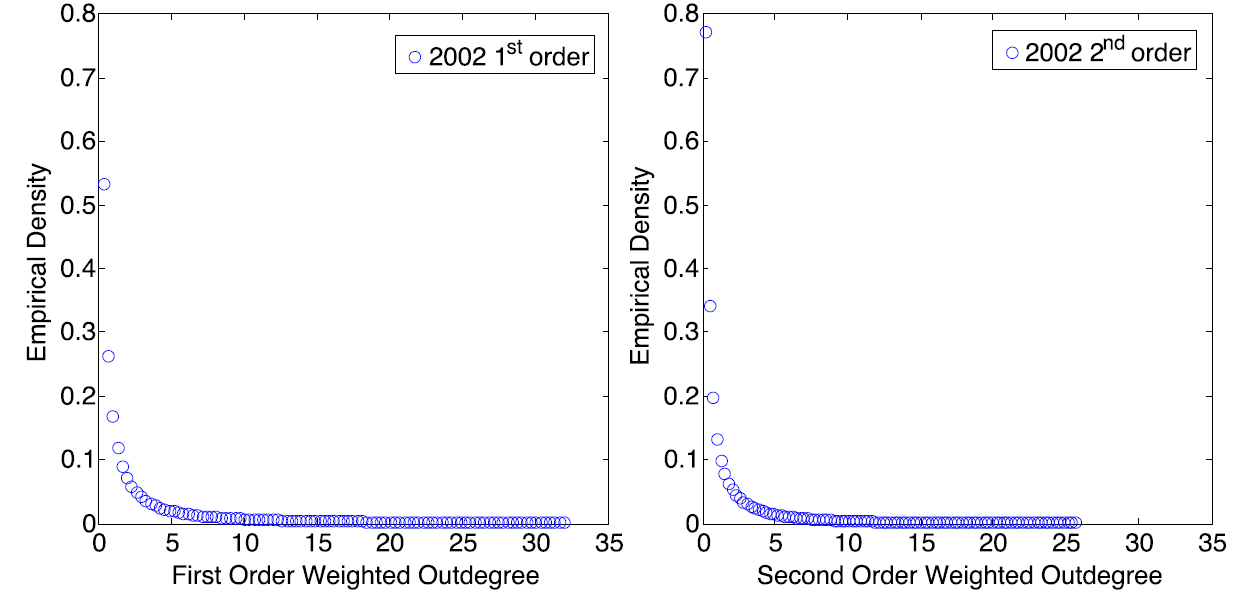
\includegraphics[scale=0.6]{5}
        \centering
    \end{figure}  

Heavy right tails, meaning that some commodities are (1) General purpose inputs used by many other sectors.
and (2) major suppliers to sectors that produce the general purpose inputs.\\[5pt]

$\implies$ The tail of the distributions is well-approximated by a power law
distribution (Pareto distribution).

\end{frame}

%%%%%%%%%%%%%%%%%%%%%%%%%
\begin{frame}{Distribution parameters estimation (1)}
    \justifying
    OLS regression of the empirical log-CCDF
    on the log-outdegree sequence are downward biased in small samples (Gabaix and Ibragimov, 2011).
    Thus implement the modified log rank–
    log size regression. Take 
    the tail of  1 minus the empirical
    cumulative distribution functions to correspond to the top 20\%
    largest sectors in terms of in an out degrees.
    \begin{align*}
        CDF_{\text{Pareto}}=1-\left(\frac{x_m}{x}\right)^\alpha
    \end{align*}
    Where $x_m$ is the scale parameter and $\alpha$ is the shape parameter.
\end{frame}
%%%%%%%%%%%%%%%%%%%%%%%%%
\begin{frame}{Distribution parameters estimation (2)}
    \justifying
    $\hat{\beta}$ and $\hat{\zeta}$ are the shape parameters for the first and 
    second-order degree distribution. (As higher is the shape parameter, more skewed is the distribution.)
    \begin{figure}[H]
        %\caption*{ Intermediate input intensity shares:}
        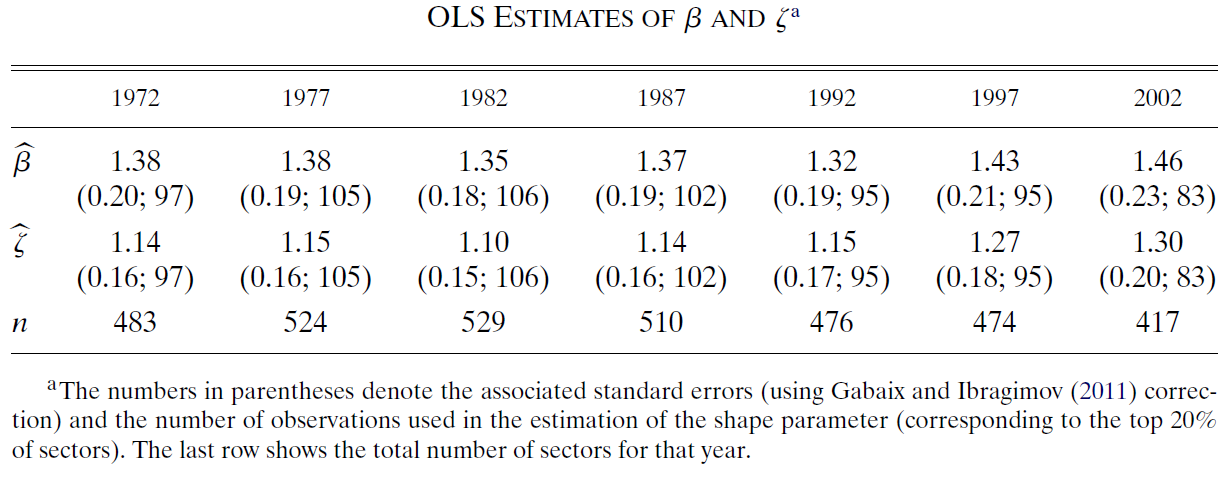
\includegraphics[scale=0.6]{7}
        \centering
\end{figure}  

High degree of asymmetry in the
U.S. economy in terms of the roles that different sectors play as direct or indirect
suppliers to others.\\
$\implies$ The interplay of
sectoral shocks and network effects leads to sizable aggregate fluctuations

\end{frame}
%%%%%%%%%%%%%%%%%%%%%%%%%
\begin{frame}{Quantitative extent of the network effects (1)}
    \justifying
Aggregate effects of sectoral shocks: Compute $||\nu_{n}||_2$
for the U.S. input–output matrix at different levels of 
aggregation and for different years.

\begin{figure}[H]
    %\caption*{ Intermediate input intensity shares:}
    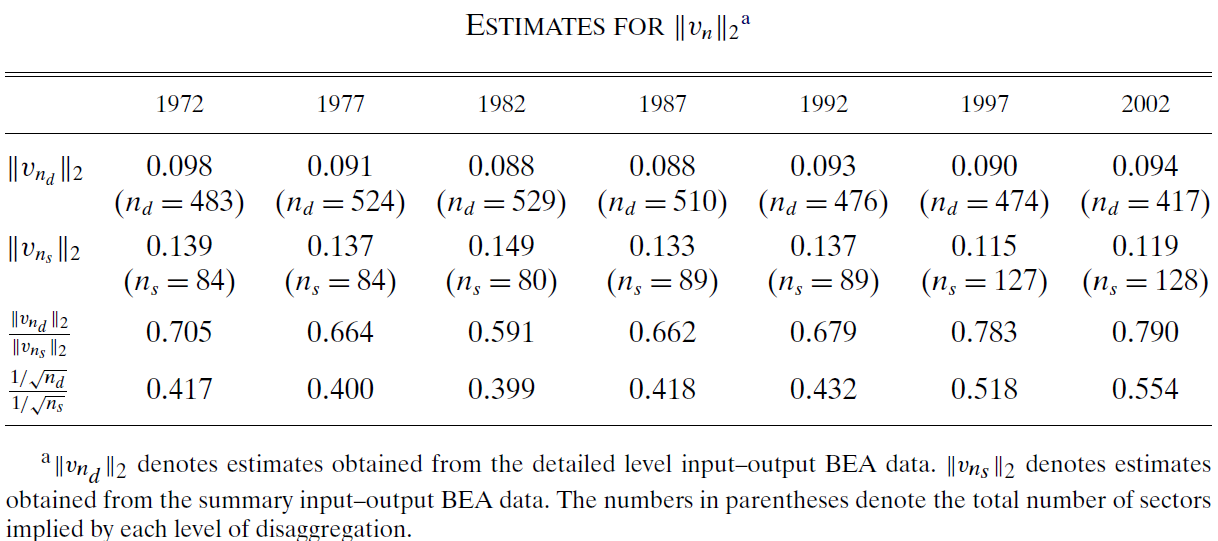
\includegraphics[scale=0.5]{8}
    \centering
\end{figure}  

$||\nu_{n_d}||_2$ at different years
are roughly twice as large as $1/\sqrt{n}$ (First row).\\
$\implies$ intersectoral linkages increase the impact of sectoral 
shocks by at least 2 times.\\[3pt]

The third row captures the change in the aggregate effect of sectoral shocks
from more to less aggregated data.\\
$\implies$ Taking intersectoral linkages into account
simply doubles the impact of sectoral shocks at all levels of disaggregation.
\end{frame}


%%%%%%%%%%%%%%%%%%%%%%%%%
\begin{frame}{Quantitative extent of the network effects (3)}
    \justifying
    If indeed taking intersectoral linkages into account
    simply doubles the impact of sectoral shocks at all levels of disaggregation
    the reatio will be  $\frac{1/\sqrt{n_d}}{1/\sqrt{n_s}}$.\\[5pt]

    If, on the other hand, network effects are more important at higher 
    levels of disaggregation, then we would expect that:
    \begin{align*}
        \frac{||\nu_{n_d}||_2}{||\nu_{n_s}||_2}>\frac{1/\sqrt{n_d}}{1/\sqrt{n_s}}
    \end{align*}


\end{frame}
%%%%%%%%%%%%%%%%%%%%%%%%%
\begin{frame}{Quantitative extent of the network effects (4)}
    \justifying
    The table early shows that the latter is indeed the case for all years. 
    For example, in 1972, as we move
    from the more aggregated measurement at the level of 84 sectors (at two-digit
    SIC) to an economy comprising 483 sectors (roughly at four-digit SIC), the
    standard diversification argument would imply a decline of 58\% in the role of
    sectoral shocks, whereas the actual decline observed in the data (measured by
    $\frac{||\nu_{n_d}||_2}{||\nu_{n_s}||_2}$is about 29\%.
    
\end{frame}

%%%%%%%%%%%%%%%%%%%%%%%%%




%Whereas the lower bound implied by the average shape parameter for the first-order
%degrees, $\beta = 1.38$, is $n(\beta-1)/\beta = n^{0.28}$. It is 
%noteworthy that this is not only a significantly slower rate of decay than
%$\sqrt{n}$ the rate predicted by the standard
%diversification argument.




%%%%%%%%%%%%%%%%%%%%%%%%%
\begin{frame}{Back-of-the-envelope calculation (1)}
    \justifying


    Using TFP estimations across 459 four-digit (SIC) manufacturing industries
    from the NBER productivity database between 1958 and 2005, compute
    its average standard deviation to be 0.058.\\[5pt]

    Average of the U.S. GDP accounted for by manufacturing is around 20\% for the 
    same time frame.\\[5pt]

Assuming that the manufacturing industries 
correspond to one-fifth of the GDP, the economy comprises $5 × 459 = 2295$ 
sectors. With a sector volatility of 0.06, if aggregate volatility decayed at
the rate $\sqrt{n}$, it expects it to be $0.058 / \sqrt{2295}=0.001$.\\[5pt]

\end{frame}

%%%%%%%%%%%%%%%%%%%%%%%%%

\begin{frame}{Back-of-the-envelope calculation (2)}
    \justifying
    The shape parameter for the second order degrees $\hat{\zeta} = 1.18$
    implies that aggregate volatility decays no faster than $n^{(\zeta-1) / \zeta} = n^{0.15}$. \\[10pt]
    
    Using the second-order degree distribution,
    aggregate volatility decays at the rate $n^{0.15}$, the same number would be
    $0.058/2295^{0.15}=0.018$. This corresponds to sizable aggregate fluctuations, in
    the ballpark of the approximately 2\% standard deviation of the U.S. GDP.
\end{frame}
% \begin{frame}{Motivation}
% \begin{itemize}
% \item Paper was written shortly after the 2008 Financial Crisis
% \item \textbf{Leading question:} How does the organization of the input-output network in an economy affect economic volatility?
% \item \textbf{Leading example: One sector}
%   \begin{itemize}
%   \item If there's one sector and one firm, then any shock to that firm shuts down the entire economy.
%     \item But if we send $n_{\text{firms}} \to \infty$ then shocks to individual firms become unimportant, and the economy is resilient to uncorrelated shocks.
%     \end{itemize}
%   \item \textbf{Leading Counterexample: Automakers during 2008}
%     \begin{itemize}
%     \item Some suppliers make small but important parts for all the carmakers
%     \item If one of these small companies collapses, there's a chance that none of the carmakers will be able to continue making cars
%       \item Ford asked congress to support Chrysler and GM so that their mutual suppliers wouldn't experience any disruptions
%     \end{itemize}
%     \item \textbf{Research Question: } Can we write down a network model of these interactions to generalize this insight? And can we fit this model to actual input/output data from the US?
%       \item \rd{NB we can put figures 1--3 on slides to show the 2 leading examples of symmetric networks, and then the actual 1997 network to show that it exhibits meaningful asymmetry.}
% \end{itemize}
% \end{frame}
\begin{frame}{Model}
  
\section{Model}

{\bf Household preferences} 
\begin{align*}
  u(c_1,c_2,\ldots ,c_n)=A \prod \limits_{i=1}^n c_i^{\frac{1}{n}}
\end{align*}

{\bf Sector production functions:} each good produced by competitive sector; can be either consumed or used by other sectors as an input
\begin{align*}
  x_i=z_i^\alpha l_i^\alpha \prod \limits_{j=1}^n x_{ij}^{(1-\alpha)w_{ij}}
\end{align*}

\begin{itemize}
  \item $x_{ij}$: Amount of commodity $j$ used in the production of good $i$
  \vitem $w_{ij}$: Share of good $j$ in total input use of firms in sector $i$
    \begin{itemize}
    \item 
      \gr{Correspond to the entries in input-output tables}
    \end{itemize}
  \vitem $z_i$: Idiosyncratic productivity shock to sector $i$. Independent across
  sectors and  $\varepsilon \equiv \log(z_i) \sim F_i$.
\end{itemize}
\end{frame}
%
\begin{frame}{Model}
  \begin{assumption}[Assumption 1]
    Input shares of all sectors add up to 1: $\sum \limits_{j=1}^n w_{ij}=1 \ \ \forall \ i$. 
  \end{assumption}
  \begin{itemize}
\item Can summarize the structure of intersectoral trade with the input-output matrix $W$, which has entries $w_{ij}$.
\vitem Economy is completely specified by the tuple
  \[
\mathcal{E} = (\mathcal{I}, W, \{F_i\}_{i \in \mathcal{I}}),\quad \mathcal{I} \text{ is the number of sectors} 
\]
% where $\mathcal{I}$ is the number of sectors.
\vitem Can equivalently represent the economy as a weighted directed graph on $n$ vertices, 
  \begin{itemize}
  \item each vertex corresponds to a sector
    \vitem A directed edge $(j, i)$ with weight $w_{ij}>0$ is present from
vertex $j$ to vertex $i$ if sector $j$ is an input supplier to sector $i$.
  \end{itemize}
 
\end{itemize}
% W with entries $w_{ij}$. Thus, the economy is completely specified by the tuple
% $\varepsilon = (I, W, F_i)$, where $I$  denotes the set of sectors.\\

% Intersectoral network of the economy: weighted graph on $n$ vertices, where
% each vertex corresponds to a sector
% in the economy, and a directed edge $(j, i)$ with weight $w_{ij}>0$ is present from
% vertex $j$ to vertex $i$ if sector $j$ is an input supplier to sector $i$.\\
\end{frame}
%
\begin{frame}{Model}
% Weighted outdegree:  Of sector i as the
% share of sector i output in the input supply of the entire economy normalized
% by constant $ 1-\alpha $ : $d_i \sum \limits_{j=1}^n w_{ij}$.\\
  \begin{definition}[Weighted Outdegree of sector $i$]
    Share of sector $i$'s output in the input supply of the entire economy, normalized by $1 - \alpha$,
    \[
d_i \equiv \sum^n_{j = 1} w_{ji}.
    \]
  \end{definition}
  \begin{itemize}
  \vitem  When all nonzero edge weights are identical, the outdegree of vertex $i$ is proportional to the number of sectors it is a supplier for.
  \end{itemize}
\end{frame}
%
\begin{frame}{Competitive Equilibrium}

The competitive equilibrium of the economy can be represented by value added:
\begin{align}
  y = \log (GDP) = \nu' \varepsilon
\end{align}

\begin{definition}[Influence Vector]
  \[
    \nu=\frac{\alpha}{n}[I-(1-\alpha)W']^{-1}
  \]
\end{definition}
\begin{itemize}
\item Aggregate output is a linear combination of log sectoral shocks with coefficients determined by the influence vector.
\vitem Aggregate output depends on the intersectoral network of the economy
through the Leontief inverse $[I - (1 - \alpha) W^\prime]^{-1}$.
\vitem Influence vector also  captures
how sectoral productivity shocks propagate downstream to other sectors
through the input–output matrix.
\end{itemize}
\end{frame}
%
\begin{frame}{Model---Influence Vector}
  \begin{itemize}
  \item The influence vector can also be interpreted as a centrality measure.
  \vitem Central sectors in the network representation of the economy play a more important role in determining aggregate output.
  \vitem 
$\nu$ is also the sales vector of the economy in the sense that the $i$th element of the influence vector is equal to the equilibrium
share of sales of sector $i$:
\begin{align}
  \nu_i=\frac{p_ix_i}{\sum \limits_{j=1}^np_jx_j}
\end{align}
  \end{itemize}
\end{frame}
%
\begin{frame}{Adding Network Structure}
  \begin{itemize}
  \item Focus on a sequence of economics where the number of sectors increases
    \vitem Characterize how the \gr{structure} of the intersectoral network affects aggregate fluctuations
    \vitem Sequence of economies $\{\mathcal{E}_n\}_{n \in \mathbb{N}}$; economy $n$ is
    \[
\mathcal{E} = (\mathcal{I}_n, W_n, \{F_{in}\}_{i \in \mathcal{I}_n})
    \]
    \vitem Since the total supply of labor is normalized to 1, increasing $n$ (number of sectors) means disaggregating the structure of the economy
  \end{itemize}
\end{frame}
%
\begin{frame}{Adding Network Structure---Notation and Assumptions}
  \begin{itemize}
  \item $\{y_n\}_{n \in \mathbb{N}}$ and $\{\nu_n\}_{n \in \mathbb{N}}$ are aggregate outputs and influence vectors
    \vitem $w_{ij}^n$ and $d_i^n$ are elements of the intersectoral matrix $W_n$ and the degree of sector $i$
    \vitem $\{\varepsilon_n\}_{n \in \mathbb{N}}$ is the sequence of vectors of (log) sectoral shocks
  \end{itemize}
  \begin{assumption}[Assumption 2]
    Given a sequence of economies $\mathcal{E}_{n \in \mathbb{N}}$, for any sector $i \in \mathcal{I}_n$ and all $n \in \mathbb{N}$,
    \begin{enumerate}
    \item[(a)] $\mathbb{E} \varepsilon_{in} = 0$
      \item[(b)] $\var (\varepsilon_{in}) = \sigma^2_{in} \in (\underline{\sigma}^2, \overline{\sigma}^2)$, where $0 < \underline{\sigma} < \overline{\sigma}$ are independent of $n$.
    \end{enumerate}
  \end{assumption}
\end{frame}
%
\begin{frame}{Aggregate Volatility}
  \begin{itemize}
  \item Assumption 2(a) and independent sectoral shocks imply that we can write \gr{aggregate volatility} as
    \[
      (\var y_n)^{1/2} = \sqrt{\sum^n_{i  = 1} \sigma^2_{in} \nu^2_{in}}.
    \]
    \vitem For any sequence of economies satisfying Assumption 2(b),
    \[
(\var y_n)^{1/2} = \Theta (\| \nu_n \|_2).
    \]
    \vitem Aggregate volatility scales with the Euclidian norm of the influence vector as the economy becomes disaggregated.
    \vitem The rate of decay of aggregate volatility may not be equal to $\sqrt{n}$ (the standard prediction from the diversification argument).
    \vitem If $\|\nu\|_2$ is bounded away from zero for all $n$, then aggregate volatility does \rd{not} disappear as $n \to \infty$.
  \end{itemize}
\end{frame}
%
\begin{frame}{Asymptotic Distributions}
  \begin{theorem}[Theorem 1]
    Consider a sequence of economies $\left\{\mathcal{E}_{n}\right\}_{n \in \mathbb{N}}$ and assume that $\mathbb{E} \varepsilon_{i n}^{2}=\sigma^{2}$ for all $i \in \mathcal{I}_{n}$ and all $n \in \mathbb{N}$
    \begin{enumerate}
    \item[(a)]
 If $\left\{\varepsilon_{\text {in }}\right\}$ are normally distributed for all $i$ and all $n$, then $\frac{1}{\left\|v_{n}\right\|_{2}} y_{n} \stackrel{d}{\longrightarrow}$ $\mathcal{N}\left(0, \sigma^{2}\right)$
\item[(b)] Suppose that there exist constant $a>0$ and random variable $\bar{\varepsilon}$ with bounded variance and cumulative distribution function $\bar{F}$, such that $F_{\text {in }}(x)<$ $\bar{F}(x)$ for all $x<-a$, and $F_{\text {in }}(x)>\bar{F}(x)$ for all $x>a .$ Also suppose that $\frac{\left\|v_{n}\right\|_{\infty}}{\left\|v_{n}\right\|_{2}} \longrightarrow 0 .$ Then $\frac{1}{\left\|v_{n}\right\|_{2}} y_{n} \stackrel{d}{\longrightarrow} \mathcal{N}\left(0, \sigma^{2}\right)$
\item[(c)] Suppose that $\left\{\varepsilon_{\text {in }}\right\}$ are identically, but not normally distributed for all $i \in \mathcal{I}_{n}$ and all $n .$ If $\frac{\left\|v_{n}\right\|_{\infty}}{\left\|v_{n}\right\|_{2}}>0$, then the asymptotic distribution of $\frac{1}{\left\|v_{n}\right\|_{2}} y_{n}$, when it exists, is nonnormal and has finite variance $\sigma^{2}$.
    \end{enumerate}
  \end{theorem}
\end{frame}
%
\begin{frame}{First-Order Interconnections}
  \begin{itemize}
  \item Characterize the rate of decay of aggregate volatility in terms of the \gr{structural properties} of the intersectoral network.
    \vitem First result: The extent of asymmetry between sectors shapes the relationship between sectoral shocks and aggregate volatility.
  \end{itemize}
  \begin{definition}[Coefficient of Variation]
     Given an economy $\mathcal{E}_{n}$ with sectoral degrees $\left\{d_{1}^{n}, d_{2}^{n}, \ldots, d_{n}^{n}\right\}$, the coefficient of variation is
$$
\mathrm{CV}_{n} \equiv \frac{1}{\bar{d}_{n}}\left[\frac{1}{n-1} \sum_{i=1}^{n}\left(d_{i}^{n}-\bar{d}_{n}\right)^{2}\right]^{1 / 2}
$$
where $\bar{d}_{n}=\left(\sum_{i=1}^{n} d_{i}^{n}\right) / n$ is the average degree.
  \end{definition}
\end{frame}
%
\begin{frame}{First-Order Interconnections}
  \begin{theorem}[Theorem 2]
    Given a sequence of economies $\left\{\mathcal{E}_{n}\right\}_{n \in \mathbb{N}}$, aggregate volatility satisfies
    \[\quad\left(\operatorname{var} y_{n}\right)^{1 / 2}=\Omega\left(\frac{1}{n} \sqrt{\sum_{i=1}^{n}\left(d_{i}^{n}\right)^{2}}\right)\]
    and
    \[\quad\left(\operatorname{var} y_{n}\right)^{1 / 2}=\Omega\left(\frac{1+\mathrm{CV}_{n}}{\sqrt{n}}\right).
    \]
  \end{theorem}
  \begin{itemize}
  \item High variability in degree sequence of intersectoral network $\implies$ high variability in effect of shocks on aggregate output.
    \vitem High CV $\implies$  few sectors are responsible for most inputs.
    \vitem Low productivity $\implies$ low productivity in downstream sectors.
    \vitem Aggregate volatility decays slower than $\sqrt{n}$.
  \end{itemize}
\end{frame}
%
\begin{frame}{Interpreting Theorem 2}
  \begin{definition}[Power Law Degree Sequence]
     A sequence of economies $\left\{\mathcal{E}_{n}\right\}_{n \in \mathbb{N}}$ has a power law degree sequence if there exist a constant $\beta>1$, a slowly varying function $L(\cdot)$ satisfying $\lim _{t \rightarrow \infty} L(t) t^{\delta}=\infty$ and $\lim _{t \rightarrow \infty} L(t) t^{-\delta}=0$ for all $\delta>0$, and a sequence of positive numbers $c_{n}=\Theta(1)$ such that, for all $n \in \mathbb{N}$ and all $k<d_{\max }^{n}=\Theta\left(n^{1 / \beta}\right)$, we have
$$
P_{n}(k)=c_{n} k^{-\beta} L(k)
$$
where $P_{n}(k) \equiv \frac{1}{n}\left|\left\{i \in \mathcal{I}_{n}: d_{i}^{n}>k\right\}\right|$ is the empirical counter-cumulative distribution function and $d_{\max }^{n}$ is the maximum degree of $\mathcal{E}_{n}$.
  \end{definition}
  \begin{itemize}
  \item Look at the special case where the intersectoral networks have power law degree sequences.
    \vitem The first part of Theorem 2 says that aggregate volatility is higher in economies whose degree sequences have ``heavier tails''.
  \end{itemize}
\end{frame}
%
\begin{frame}{Interpreting Theorem 2}
  \begin{corollary}[Corollary 1]
     Consider a sequence of economies $\left\{\mathcal{E}_{n}\right\}_{n \in \mathbb{N}}$ with a power law degree sequence and the corresponding shape parameter $\beta \in(1,2) .$ Then, aggregate volatility satisfies
$$
\left(\operatorname{var} y_{n}\right)^{1 / 2}=\Omega\left(n^{-(\beta-1) / \beta-\delta}\right)
$$
where $\delta>0$ is arbitrary.
  \end{corollary}
  \begin{itemize}
  \item If the degree sequence of the intersectoral network exhibits heavy tails, aggregate volatility decreases at a much slower rate than predicted by the diversification argument.
    \vitem Note that so far the authors have only provided a \rd{lower bound} on the rate at which aggregate volatility vanishes.
    \vitem Higher-order structural properties of the intersectoral network can still prevent output volatility from decaying at rate $\sqrt{n}$.
  \end{itemize}
\end{frame}
%
\begin{frame}{Second-Order Interconnections and Cascades}
  \begin{itemize}
  \item First-order interconnections provide little information about how shocks to a sector affect the downstream customers of downstream customers of the affected sector, etc.
    \vitem The next theorem provides a lower bound on the decay rate of aggregate volatility in terms of \gr{second-order} interconnections in the intersectoral network.
    \begin{definition}[Definition 3---$2$nd-Order Interconnectivity Coefficient]
       The second-order interconnectivity coefficient of economy $\mathcal{E}_{n}$ is
$$
\tau_{2}\left(W_{n}\right) \equiv \sum_{i=1}^{n} \sum_{j \neq i} \sum_{k \neq i, j} w_{j i}^{n} w_{k i}^{n} d_{j}^{n} d_{k}^{n}.
$$
    \end{definition}
    \item Measures extent to which high degree sectors are connected to each other via common suppliers
  \end{itemize}
\end{frame}
%
\begin{frame}{Second-Order Interactions and Cascades}
  \begin{theorem}[Theorem 3]
    Given a sequence of economies $\left\{\mathcal{E}_{n}\right\}_{n \in \mathbb{N}}$, aggregate volatility satisfies
 \[\quad\left(\operatorname{var} y_{n}\right)^{1 / 2}=\Omega\left(\frac{1}{\sqrt{n}}+\frac{\mathrm{CV}_{n}}{\sqrt{n}}+\frac{\sqrt{\tau_{2}\left(W_{n}\right)}}{n}\right)\]
  \end{theorem}
  \begin{itemize}
  \item Shows how second-order interactions, captured by $\tau_2$, affect aggregate volatility.
    \vitem Even if the empirical degree distributions of two sequences of economies are identical for all $n$, their aggregate volatilities may exhibit considerably different behaviors.
    \vitem This is a refinement of Theorem 2; it captures the notion that there is a clustering of significant sectors because they have common suppliers.
  \end{itemize}
\end{frame}
%
\begin{frame}{Interpreting Theorem 3}
  \begin{corollary}[Corollary 2]
     Suppose that $\left\{\mathcal{E}_{n}\right\}_{n \in \mathbb{N}}$ is a sequence of economies whose second-order degree sequences have power law tails with shape parameter $\zeta \in$ $(1,2)($ cf. Definition 2). Then, aggregate volatility satisfies
$$
\left(\operatorname{var} y_{n}\right)^{1 / 2}=\Omega\left(n^{-(\zeta-1) / \zeta-\delta}\right)
$$
for any $\delta>0$.
  \end{corollary}
  \begin{itemize}
  \item If the distributions of second-order degrees have heavy tails, aggregate volatility decreases much more slowly than predicted by diversification.
    \vitem Second-order effects may dominate first-order effects.
    \vitem If a sequence of economies has power law tails for both first- and second-order degrees, with exponents $\beta$ and $\zeta$, then the tighter bound for the decay rate of aggregate volatility is determined by $\min \{\beta, \zeta\}$.
  \end{itemize}
\end{frame}
%
\begin{frame}{Balanced Structures}
  \begin{itemize}
  \item With limited variations in the degrees of different sectors, aggregate volatility decays at rate $\sqrt{n}$.
    \begin{definition}[Definition 4---Balanced Sequence of Economics]
       A sequence of economies $\left\{\mathcal{E}_{n}\right\}_{n \in \mathbb{N}}$ is balanced if $\max _{i \in \mathcal{I}_{n}} d_{i}^{n}=$ $\Theta(1)$.
    \end{definition}
    \vitem When the intersectoral network is balanced and the role of intermediate inputs is not too large, volatility decays at rate $\sqrt{n}$.
    \vitem Other structural properties of the network cannot contribute to aggregate volatility.
    \begin{theorem}[Theorem 4]
       Consider a sequence of balanced economies $\left\{\mathcal{E}_{n}\right\}_{n \in \mathbb{N}}$. Then there exists $\bar{\alpha} \in(0,1)$ such that, for $\alpha \geq \bar{\alpha}$, (var $\left.y_{n}\right)^{1 / 2}=\Theta(1 / \sqrt{n})$.
    \end{theorem}
  \end{itemize}
\end{frame}
%
\begin{frame}{Interpreting Theorem 4}
  \begin{itemize}
  \item Theorem 4 is both an aggregation and an irrelevance result for balanced economies.
    \vitem As an aggregation result, it suggests observational equivalence between the one-sector economy and any balanced multi-sector economy.
    \vitem As an irrelevance result, it shows that different input-output matrices generate roughly the same volatility for balanced economies.
  \end{itemize}
\end{frame}
\end{document}

%%% Local Variables:
%%% mode: latex
%%% TeX-master: t
%%% End:
